\documentclass[12pt,twoside]{article}
\usepackage{amsmath}
\usepackage[active]{srcltx}
\usepackage{amssymb}
\usepackage{amscd}
\usepackage{makeidx}
\usepackage{amsthm}
\usepackage{algorithm}
\usepackage{amssymb, amsmath}
\usepackage[utf8]{inputenc}
\usepackage{fancyhdr}
\usepackage{graphics}
\usepackage{amsmath, amssymb}
\usepackage{amsmath}
\usepackage{listings}
\usepackage{xcolor}
\usepackage{fancyhdr}
\usepackage[active]{srcltx}
\usepackage{amsmath}
\usepackage{amssymb}
\usepackage{amscd}
\usepackage{makeidx}
\usepackage{graphicx}
\usepackage{caption}
\usepackage{url}
\usepackage{enumitem}
\usepackage{fancybox}
\usepackage{tabularx}

\renewcommand{\baselinestretch}{1}
\setcounter{page}{1}
\setlength{\textheight}{21.6cm}
\setlength{\textwidth}{14cm}
\setlength{\oddsidemargin}{1cm}
\setlength{\evensidemargin}{1cm}
\pagestyle{myheadings}
\thispagestyle{empty}
\markboth{\small{TMP(Nombre de equipo)}}{\small{Formulación del Proyecto}}
\date{} 

\begin{document}
	
	\begin{center}
		
		% Contenido izquierdo - Imagen
		\begin{minipage}{0.17\textwidth}
			\flushleft
			
\includegraphics[width=0.9\textwidth]{img/ipn_logo.png} % Ajusta esta línea
		\end{minipage}
		\begin{minipage}{.55\textwidth}
			\centering
			{\Large Instituto Politécnico Nacional}\\
			{\Large Escuela Superior de Cómputo}
		\end{minipage}
		\begin{minipage}{0.17\textwidth}
			\flushright
			
\includegraphics[width=0.9\textwidth]{img/escom_logo} % Ajusta esta línea
		\end{minipage}			
	\end{center}
	
	
	\centerline{\bf Ingeniería en Inteligencia Artificial, Análisis y diseño de sistemas}
	
	\centerline{\bf Sem: 2024-2, 4BM2, TMP(Nombre de la actividad), Fecha: 27-06-24\\\\}
	
	\centerline{}
	
	%\centerline{}
	
	
	\begin{center}
		\Large{\textsc{Ecos del alma: Prototipo de juego rogue like con interacción jugador-NPC dinámica}} 
	\end{center}
	\centerline{}
	\centerline{\bf {\textit{Presentan}}}
	\centerline{}
	\centerline{\bf {Angeles López Erick Jesse\footnote{eangelesl1700@alumno.ipn.mx}}}
	\centerline{\bf {Corona Anchondo José Antonio\footnote{jcoronaa1900@alumno.ipn.mx}}}
	\centerline{\bf {	Espinosa Martínez José Carlos\footnote{jespinosam1900@alumno.ipn.mx}}}
	\centerline{\bf {Esquivel García Thania Paola\footnote{tesquivelg2000@alumno.ipn.mx}}}
	
	
	
	\newtheorem{Theorem}{\quad Theorem}[section]
	
	\newtheorem{Definition}[Theorem]{\quad Definition}
	
	\newtheorem{Corollary}[Theorem]{\quad Corollary}
	
	\newtheorem{Lemma}[Theorem]{\quad Lemma}
	
	\newtheorem{Example}[Theorem]{\quad Example}
	
	\bigskip
	
	\bigskip
	
	\textbf{Resumen:}  \\ 
	
	{\bf Palabras Clave:} \\
	
	\clearpage
	
	\tableofcontents
		
	\clearpage
		
	\section{Introducción}
	
	\clearpage
	\section{Estado del arte}%Videjuegos y aplicaciones que simulen este comportamiento conversacional
	Algunos juegos y aplicaciones similares son:
	\begin{enumerate}[noitemsep]
		\item Videojuego \textit{Hades} desarrollado por Supergiant Games \cite{game:hades}. 

		\item Videojuego \textit{Celeste} desarrollado por Maddy Makes Games \cite{game:celeste}

		\item Videojuego \textit{Hollow Knight} desarrollado por Team Cherry \cite{game:hollow}
		
		\item Videojuego \textit{Coffee Talk} desarrollado por Toge Productions \cite{game: coffee}
		
		\item Aplicación \textit{character.ai} desarrollada por Character Technologies, Inc. \cite{app: character}
	\end{enumerate}
	
	\begin{table}[H]
		\centering
		\begin{tabular}{|c|p{9cm}|}
			\hline
			\textbf{Producto} & \multicolumn{1}{c|}{\textbf{Características}} \\ \hline
			 Hades &  Juego \textit{rogue like}  con niveles generados proceduralmente conectando diferentes habitaciones.\\ \hline
			 
			 Celeste &  Juego de plataformas con jugabilidad invariable, conversación ocasional con NPC y mecanicas de movimiento avanzadas. \\ \hline
			 
			 Hollow knight &   Juego \textit{metroidvania} con poca interacción conversacional, mecanicas de movimiento y combate avanzada. \\ \hline
			 
			 Coffee talk &   Juego de genero novela visual y aventura conversacional, las respuestas (limitadas por el juego) definen las relaciones con los NPC. \\ \hline
			 
			 character.ai&   Aplicación online para diseñar o conversar con bots inteligentes y personificados unicamente mediante lineas de texto. \\ \hline
		\end{tabular}
		\caption{Resumen de juegos y aplicaciones similares}
		\label{table: aplicaciones}
	\end{table} 
	
	\clearpage
	\section{Justificación}
	
	
	
	\clearpage
	\section{Objetivo general}
	Desarrollar el prototipo de un videojuego \textit{rogue like} con generación de niveles procedurales e interacción jugador-NPC desde el teclado mediante análisis de texto, simulación de emociones y toma de decisiones.
	
	\section{Objetivos particulares}
	
	\begin{itemize}
		\item Desarrollar un generador de niveles procedurales con habitaciones prediseñadas estilo \textit{dungeon}.
		\item Diseñar, para los NPC, factores de personalidad y flujos conversacionales.
		\item Desarrollar  un modelo  de procesamiento de lenguaje natural para analizar respuestas del jugador.
		\item Recopilar conversaciones y respuestas entre el jugador y los NPC.
	\end{itemize}
	
	\clearpage
	\section{TMP(Capitulos de contexto)}
	
	\clearpage
	\section{Análisis}
	
	\subsection{Metodología}

	La metodología para el proyecto es el modelo de entrega por etapas. Este modelo nos permite planificar y diseñar componentes de forma individual siempre orientados a los mismos objetivos.

	El videojuego puede tener productos funcionales en las primeras etapas de desarrollo. Es por esto por lo que el modelo de entrega por etapas maximiza la productividad, permitiendo desarrollar elementos adicionales en cada una de sus etapas. 
	
	Estas implementaciones pueden ser desde niveles adicionales, mecánicas nuevas, correcciones y expansiones del mismo proyecto, permitiendo diversidad y adaptabilidad a pequeños cambios.
	
	\subsection{Tecnología}	% Herramientas, software, lenguajes de programación que seran utilizados para el desarrollo

	\subsubsection{Motor de desarrollo Unity}
	Unity es un motor y una plataforma de desarrollo de videojuegos para diseñar contenido audiovisual en 2D y 3D. Permite a programadores, artistas, arquitectos, diseñadores, cineastas, etc. diseñar, construir y desplegar sus propios proyectos en diferentes dispositivos \cite{app: unity}.

Se opta por Unity sobre otras herramientas populares en el mercado como lo son Godot, Unreal Engine y Game Maker por las siguientes razones:

\begin{itemize}
	\item Unity es el motor estandarizado para el desarrollo de proyectos nuevos, con una amplia comunidad y numerosos recursos disponibles.
	\item El juego requiere de \textit{sprites} estilo \textit{pixel art} que pueden ser segmentados y animados fácilmente mediante el IDE de Unity.
	\item El juego no requiere mucho procesamiento en los gráficos, por lo que Unity resulta una opción más cómoda y eficiente frente a Unreal Engine, que está más orientado a gráficos de alta calidad y realismo.
	\item Unity ofrece una excelente documentación y soporte técnico, lo que facilita la resolución de problemas y la implementación de características avanzadas.
	\item El editor visual de Unity es intuitivo y facilita la creación de niveles y la implementación de mecánicas de juego complejas sin requerir conocimientos avanzados en programación.
	\item Unity proporciona un excelente sistema de física y colisiones que puede ser aprovechado para crear interacciones detalladas y precisas en el juego.
\end{itemize}

	\subsubsection{Lenguaje de programación C\#}
	Lenguaje de programación utilizado comúnmente en Unity para el desarrollo de videojuegos. Es un lenguaje orientado a objetos con un sistema de gestión automática de memoria  \cite{lan: c_sharp}.
	
	\subsubsection{Lenguaje de programación Prolog}
	Lenguaje de programación basado en declaración de hechos, establecimiento de reglas e inferencia de preguntas. Permite generar una base de conocimientos relacionando diferentes hechos  mediante secuencias lógicas enlazadas \cite{lan: prolog}.
	
	Su uso sera como una librería a la cual podremos acceder desde C\# para generar la base de conocimientos y la generación de inferencias. 
	
	\subsubsection{MongoDB}
	MongoDB es un sistema gestor de base de datos NoSQL orientado a documentos con estructuras BSON y esquematización dinámica.

	\begin{itemize}
	\item Incluye medidas de seguridad robustas:
		\begin{itemize}
			\item \textbf{Autenticación:} Registro mediante credenciales de Atlas, GitHub o Google, lo que garantiza un acceso controlado y seguro a la base de datos.
			\item \textbf{Autorización:} Creación y asignación de roles y permisos para controlar el acceso y las operaciones que cada usuario puede realizar.
			\item \textbf{Auditoría:} Monitoreo detallado de acciones en el entorno de MongoDB, permitiendo rastrear cambios y accesos para garantizar la seguridad y el cumplimiento de normas.
			\item \textbf{Encriptación:} Protección de datos tanto en reposo como en tránsito, asegurando que la información sensible esté siempre protegida contra accesos no autorizados.
		\end{itemize}
	\item Ofrece tiempos de consulta reducidos en comparación con sistemas relacionales, lo que mejora significativamente el rendimiento en aplicaciones con grandes volúmenes de datos.
	\item Escalabilidad horizontal y vertical, permitiendo ajustar la capacidad de la base de datos según las necesidades del proyecto. Esto es especialmente útil para aplicaciones que requieren manejar grandes cantidades de datos y usuarios.
	\item Herramientas de transcripción de modelos SQL a NoSQL, facilitando la migración y la integración de bases de datos existentes.
	\item Conectividad con diferentes herramientas y sistemas de gestión, proporcionando flexibilidad y facilitando la integración con otros componentes del ecosistema tecnológico del proyecto.
	\item Integración con frameworks de desarrollo populares, lo que facilita su uso en diversas aplicaciones y entornos de desarrollo \cite{lan: mongo}.
\end{itemize}


	\subsubsection{Star UML}
	Herramienta de modelado UML desarrollado por MKLab. Es una de las herramientas UML más populares en el mundo. Se ha descargado más de 4 millones de personas y se utiliza en más de 150 países.
	
	Es compatible con los principales lenguajes de programación como Java, C\# y C ++. Puede generar códigos fuente de sus modelos o construir un modelo a partir de código fuente mediante ingeniería	inversa \cite{app: star}. 
	
	\subsubsection{Pixilart}
	Aplicación web y red social que permite diseñar, modificar, publicar y compartir imagenes estilo \textit{pixel art} de forma gratuita \cite{app: pixilart}.
	
	Esta plataforma nos permite crear grupos privados donde se puedan compartir y editar diferentes diseños. Cuenta con un amplio abanico de herramientas para colorear y dibujar en cuadricula, permitiendo formatos de alta calidad.
	
	\clearpage
	\subsection{Requerimientos}
	
	\subsubsection{Requerimientos funcionales}
	\textbf{Respecto a la jugabilidad} 
	\begin{enumerate}[label=RF\arabic*]
		\item Al iniciar, el juego muestra el menú principal con opciones para cargar partida, borrar partida, salir y acceder a la configuración.
		\item El jugador controla las acciones y las interacciones del personaje jugable.
		\item Al inicio, el juego sitúa al jugador y a un número exacto de NPC en el \textit{respawn}.
		\item El jugador comienza un intento de progresión.
		\item Cuando el jugador inicia el intento o termina un nivel previo, el juego genera de forma procedural el siguiente nivel, compuesto por un número finito de habitaciones con obstáculos.
		\item Cuando el jugador termina el último nivel, regresa al jugador al respawn.
		\item Al finalizar cada nivel, el juego presenta una habitación con un NPC.
		\item Cuando el personaje agota sus vidas, reaparece con el último NPC con el que interactuó y entra en modo ``after'' (conservando los mismos controles), y sus estadísticas se determinan con base en el flujo de conversación.
		\item Si el personaje encuentra su lugar de muerte en modo ``after'', regresa al modo normal.
		\item Si el personaje muere en modo ``after'', vuelve al \textit{respawn} con el último NPC con el que interactuó ahí, y sus estadísticas se ajustan de acuerdo con el flujo de conversación.
	\end{enumerate}	
	
	\noindent\textbf{Respecto a la configuración}
	\begin{enumerate}[label=RF\arabic*]
		\setcounter{enumi}{10}
		\item El jugador puede configurar manualmente todos los controles o elegir la configuración predeterminada.
		\item Se permite al jugador controlar el volumen general del juego, los efectos y la música.
		\item Al terminar la interacción con un personaje, el juego guarda los datos de la partida.
		\item Al volver al menú principal, el jugador guarda los datos de la partida.
	\end{enumerate}
	
	\noindent\textbf{Respecto a los controles}
	\begin{enumerate}[label=RF\arabic*]
		\setcounter{enumi}{14}
		\item \textbf{Movimiento lateral: }El personaje puede desplazarse a lo largo del plano 2D.
		\item \textbf{Salto: }El personaje efectúa un salto vertical independiente del movimiento lateral, limitado por colisiones.
		\item \textbf{Dash: }El personaje realiza un impulso rápido en la dirección elegida por el jugador, que tiene un período de enfriamiento antes de poder reutilizarse.
	\end{enumerate}
	
	\noindent\textbf{Respecto a la interacción con el entorno}
	\begin{enumerate}[label=RF\arabic*]
		\setcounter{enumi}{17}
		\item \textbf{Conversación: }El personaje puede iniciar conversaciones con NPC.
		\item \textbf{Finalizar conversación:} El jugador puede cerrar la ventana de diálogo con el NPC.
		\item \textbf{Cambio de escenario: }El personaje puede interactuar con puertas (o agujeros) para entrar, salir o cambiar de escenario.
		\item \textbf{Sistema de vidas: }El personaje pierde salud al colisionar con obstáculos y la recupera al recoger objetos de curación.
	\end{enumerate}
	
	\noindent\textbf{Respecto a la interacción con el sistema inteligente}
	\begin{enumerate}[label=RF\arabic*]
		\setcounter{enumi}{21}
		\item Cuando el jugador interactúa con un NPC, este responde según el flujo de conversación actualizado.
		\item El jugador introduce su respuesta en la conversación mediante el teclado.
		\item Con la respuesta del jugador, el juego procesa el mensaje, genera una respuesta y actualiza el flujo de conversación.
		\item El jugador tiene un número máximo de respuestas por encuentro con cada NPC.
		
	\end{enumerate}
	
	\subsubsection{Requerimientos no funcionales}
	
	\begin{enumerate}[label=RNF\arabic*]
		\item \textbf{Seguridad de Acceso: }Solo los jugadores registrados podrán acceder al juego, asegurando una experiencia segura y personalizada.
		\item \textbf{Personalización Basada en el Perfil del Jugador: }El contenido y las opciones disponibles en el juego variarán según el progreso y las acciones del jugador.
		\item \textbf{Conexión a Internet para Funcionalidades del sistema inteligente: }Se requerirá conexión a internet para acceder al servidor que contiene el sistema inteligente, permitiendo la interacción dinámica con NPC. El juego no incluirá características multiplayer online.
		\item \textbf{Mensajes de Error Claros: }Los mensajes de error serán informativos, ayudando a los jugadores a entender y resolver problemas rápidamente.
		\item \textbf{Diseño Adaptable a Diferentes Resoluciones y Plataformas de Escritorio:} El juego, diseñado exclusivamente para escritorio (Windows y macOS), adaptará su interfaz y gráficos a diferentes resoluciones de pantalla.
		\item \textbf{Usabilidad: }El juego será intuitivo y fácil de navegar, ofreciendo una experiencia agradable para un amplio rango de jugadores.
		\item \textbf{Terminología Amigable: }Se utilizará un lenguaje claro y accesible, evitando jerga complicada para facilitar la comprensión del juego.
		\item \textbf{Tiempo de Generación de Contenido Dinámico:} Contenidos como diálogos o eventos se generarán en menos de 10 segundos, manteniendo el flujo del juego.
		\item \textbf{Generación Simultánea de Contenidos: }El juego será capaz de generar múltiples elementos de juego de forma simultánea sin degradar el rendimiento.
		\item \textbf{Integridad del Contenido Generado: }Se asegurará que el contenido generado, como diálogos o eventos, sea relevante y libre de errores significativos.
		\item \textbf{Feedback Visual Durante Cargas: }Se proporcionarán indicadores de progreso durante las cargas para mantener informados a los jugadores.
		\item \textbf{Accesibilidad y Configuración de Teclado: }El juego permitirá a los usuarios configurar las teclas de acceso rápido y ajustar la sensibilidad del teclado.
		\item \textbf{Latencia Baja en la Entrada del Teclado: }Se garantizará una latencia mínima en la respuesta a las entradas del teclado.
		\item \textbf{Soporte para Atajos de Teclado: }El juego incluirá atajos de teclado intuitivos para acciones comunes.
		\item \textbf{Estilo Visual Amigable y Pixel Art: }El diseño del juego, basado en pixel art, promoverá un estilo visual amigable y atractivo, adecuado para una amplia audiencia.
		\item \textbf{Identificación Clara de Objetos y Elementos: }Tanto en el apartado visual como sonoro, los objetos y elementos importantes del juego serán fácilmente identificables, mejorando la experiencia de juego.
		\item \textbf{Juiciness en la Jugabilidad: }El juego incorpora elementos de "juiciness", ofreciendo retroalimentación inmediata y satisfactoria a las acciones del jugador a través de efectos visuales, sonoros y mecánicos que hacen que la experiencia de juego sea más dinámica y gratificante.
		
	\end{enumerate}
	
	
	\subsubsection{Requerimientos mínimos de sistema}

	\begin{table}[H]
		\centering
		\begin{tabular}{|c|l|}
			\hline
			\multicolumn{2}{|c|}{\textbf{Windows}} \\ \hline
			\textbf{Sistema operativo} & Windows  7 o mas reciente.\\ \hline
			\textbf{Procesador} &  Intel Core i3 M380. \\ \hline
			\textbf{Memoria} &  2GM de RAM. \\ \hline
			\textbf{Gráficos} &   Intel HD 4000. \\ \hline
			\textbf{DirectX} &   Versión 10. \\ \hline
			\textbf{Almacenamiento} &   1.5 GB de espacio disponible. \\ \hline
		\end{tabular}
		\caption{Requerimientos mínimos de sistema para Windows.}
		\label{table: requerimientos_windows}
	\end{table} 
	
	\begin{table}[H]
		\centering
		\begin{tabular}{|c|l|}
			\hline
			\multicolumn{2}{|c|}{\textbf{Macos}} \\ \hline
			\textbf{Sistema operativo} & Lion 10.7.5, 32/64 bits o más reciente. \\ \hline
			\textbf{Procesador} &  Intel Core i3 M380. \\ \hline
			\textbf{Memoria} &  2GM de RAM. \\ \hline
			\textbf{Gráficos} &  OpenGL 3.0 o superior. \\ \hline
			\textbf{Almacenamiento} &   1.5 GB de espacio disponible. \\ \hline
		\end{tabular}
		\caption{Requerimientos mínimos de sistema para Macos.}
		\label{table: requerimientos_mac}
	\end{table} 

	\clearpage
	\section{Diseño}
	
	\subsection{Diagrama de contexto}
	
	\begin{figure}[H]
		\centering
		\fbox{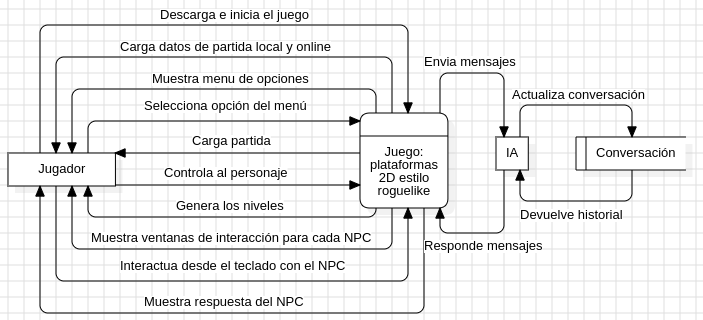
\includegraphics[width=1\textwidth]{img/contexto.png}}
		\caption{Diagrama de contexto}
		\label{diagrama: contexto}
	\end{figure}
	
	\subsection{Diagrama de flujo de datos}
	
	\begin{figure}[H]
		\centering
		\fbox{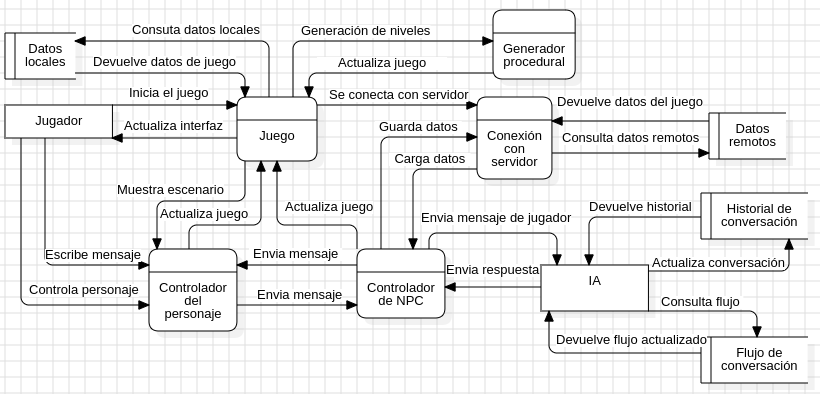
\includegraphics[width=1\textwidth]{img/flujo_datos.png}}
		\caption{Diagrama de flujo de datos}
		\label{diagrama: flujo_datos}
	\end{figure}
	
	\subsection{Diagrama de casos de uso}
	
	\begin{figure}[H]
		\centering
		\fbox{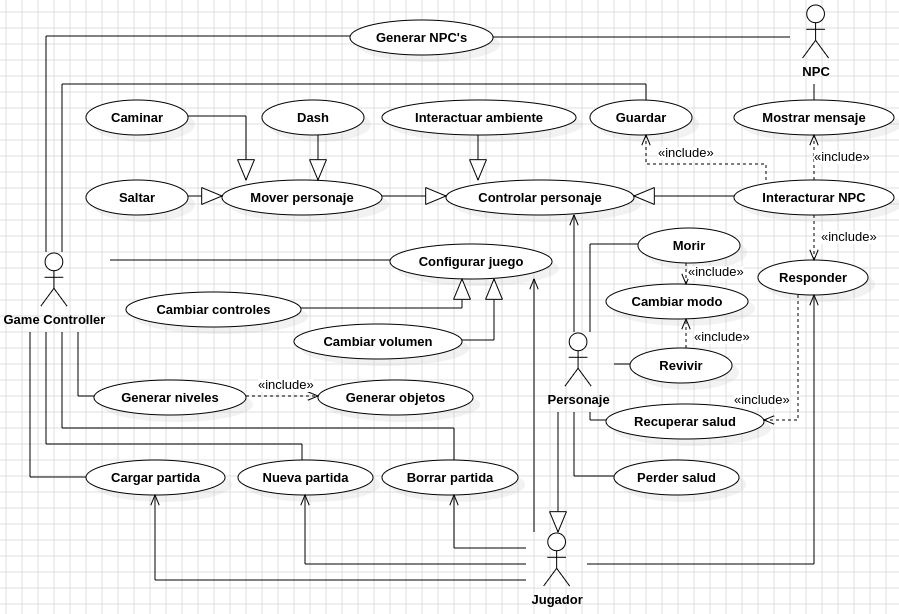
\includegraphics[width=1\textwidth]{img/casos_de_uso1.png}}
		\caption{Diagrama de casos de uso}
		\label{diagrama: casos_de_uso1}
	\end{figure}
	
	\begin{figure}[h!]
		\centering
		\fbox{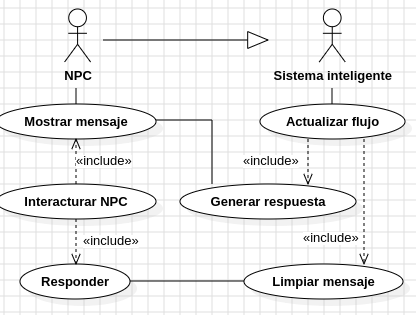
\includegraphics[width=.5\textwidth]{img/casos_de_uso2.png}}
		\caption{Diagrama de casos de uso}
		\label{diagrama: casos_de_uso2}
	\end{figure}
	
	
	
	\subsubsection{Especificaciones de casos de uso del jugador(personaje)}
	
	%Nueva partida
	\begin{figure}[H]
		\centering
		\fbox{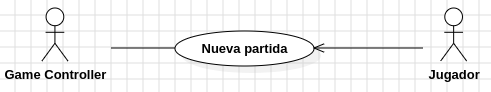
\includegraphics[width=.75\textwidth]{img/casos/nueva_partida.png}}
		\caption{Caso de uso:  Nueva partida}
		\label{diagrama: caso: nueva_partida}
	\end{figure}
	
	\begin{table}[H]
		\centering
		\begin{tabularx}{\textwidth}{|p{0.3\textwidth}|p{0.3\textwidth}|p{0.3\textwidth}|}
			\hline
			\textbf{CASO DE USO} & \multicolumn{2}{|l|}{Nueva partida} \\ \hline
			
			\textbf{ACTOR} & \multicolumn{2}{|l|}{Jugador} \\ \hline
			
			\textbf{DESCRIPCIÓN} & \multicolumn{2}{|>{\raggedright\arraybackslash}X|}{El jugador inicia una nueva partida en un `slot' disponible.} \\ \hline
		
			\textbf{PRECONDICIÓN} & \multicolumn{2}{|l|}{Ninguna} \\ \hline
			
			\textbf{FLUJO BÁSICO} & \textbf{ACTOR} & \textbf{SISTEMA} \\ \hline
			& 
			1. Presiona el botón de `Nueva partida' en el menú principal. \newline
			3. Selecciona un `slot' disponible.
			& 
			2. Muestra `slots' de almacenamiento. \newline
			4. Crea datos de partida e inicia el juego.
			\\ \hline
			
			\textbf{FLUJO ALTERNO} & \textbf{ACTOR} & \textbf{SISTEMA} \\ \hline
			
			1. Sin `slots' de almacenamiento: Cancelar.
			& 
			1. Presiona el botón de `Nueva partida' en el menú principal. \newline
			3. Selecciona un `slot' no disponible. \newline
			5. Selecciona la opción de cancelar.
			&
			2. Muestra `slots' de almacenamiento. \newline
			4. Mensaje de advertencia para sobrescribir datos o cancelar. \newline
			6. Regresa al menú principal.
			\\ \hline
			
			\textbf{FLUJO ALTERNO} & \textbf{ACTOR} & \textbf{SISTEMA} \\ \hline
			
			2. Sin `slots' de almacenamiento: Cancelar.
			& 
			1. Presiona el botón de `Nueva partida' en el menú principal. \newline
			3. Selecciona un `slot' no disponible. \newline
			5. Selecciona la opción de sobrescribir.
			&
			2. Muestra `slots' de almacenamiento. \newline
			4. Mensaje de advertencia para sobrescribir datos o cancelar. \newline
			6. Borra datos de partida pasada, crea datos de partida e inicia el juego.
			\\ \hline
			
			\textbf{POSTCONDICIÓN} & \multicolumn{2}{|l|}{Ninguna} \\ \hline
		\end{tabularx}
		\caption{Descripción del caso de uso: Nueva partida.}
		\label{table:caso_nueva_partida}
	\end{table}
	
	%Cargar partida
	\begin{figure}[H]
		\centering
		\fbox{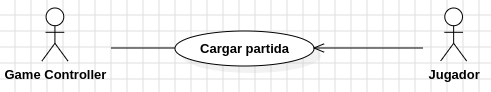
\includegraphics[width=.75\textwidth]{img/casos/cargar_partida.png}}
		\caption{Caso de uso: Cargar partida}
		\label{diagrama: caso: cargar_partida}
	\end{figure}
	
	\begin{table}[H]
		\centering
		\begin{tabularx}{\textwidth}{|p{0.3\textwidth}|p{0.3\textwidth}|p{0.3\textwidth}|}
			\hline
			\textbf{CASO DE USO} & \multicolumn{2}{|l|}{Cargar partida} \\ \hline
			
			\textbf{ACTOR} & \multicolumn{2}{|l|}{Jugador} \\ \hline
			
			\textbf{DESCRIPCIÓN} & \multicolumn{2}{|>{\raggedright\arraybackslash}X|}{El jugador carga los datos de la partida guardada e inicia el juego.} \\ \hline
			
			\textbf{PRECONDICIÓN} & \multicolumn{2}{|l|}{Nueva partida} \\ \hline
			
			\textbf{FLUJO BÁSICO} & \multicolumn{1}{|c|}{\textbf{ACTOR}} & \multicolumn{1}{|c|}{\textbf{SISTEMA} } \\ \hline
			& 
			1. Selecciona el `slot' de partida.
			&
			2. Carga datos de partida, e inicia el juego.
			 \\ \hline
			
			\textbf{POSTCONDICIÓN} & \multicolumn{2}{|l|}{Ninguna} \\ \hline
		\end{tabularx}
		\caption{Descripción del caso de uso: Cargar partida }
		\label{table: caso: cargar_partida}
	\end{table}
	
	%Borrar partida
	\begin{figure}[H]
		\centering
		\fbox{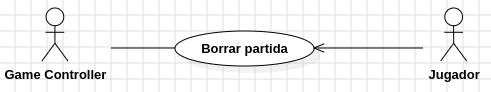
\includegraphics[width=.75\textwidth]{img/casos/borrar_partida.png}}
		\caption{Caso de uso: Borrar partida.}
		\label{diagrama: caso: borrar_partida}
	\end{figure}
	
	\begin{table}[H]
		\centering
		\begin{tabularx}{\textwidth}{|p{0.3\textwidth}|p{0.3\textwidth}|p{0.3\textwidth}|}
			\hline
			\textbf{CASO DE USO} & \multicolumn{2}{|l|}{Borrar partida} \\ \hline
			
			\textbf{ACTOR} & \multicolumn{2}{|l|}{Jugador} \\ \hline
			
			\textbf{DESCRIPCIÓN} & \multicolumn{2}{|>{\raggedright\arraybackslash}X|}{El jugador elimina los datos guardados de una partida.} \\ \hline
			
			\textbf{PRECONDICIÓN} & \multicolumn{2}{|l|}{Nueva partida} \\ \hline
			
			\textbf{FLUJO BÁSICO} & \multicolumn{1}{|c|}{\textbf{ACTOR}} & \multicolumn{1}{|c|}{\textbf{SISTEMA} } \\ \hline
			& 
			1. Selecciona el botón de eliminar `slot' de partida. \newline
			3. Selecciona eliminar los datos.
			&
			2. Mensaje de advertencia para eliminar o cancelar. \newline
			4. Elimina permanente los datos de partida del `slot'.
			 \\ \hline
			
			\textbf{FLUJO ALTERNO} & \multicolumn{1}{|c|}{\textbf{ACTOR}} & \multicolumn{1}{|c|}{\textbf{SISTEMA} } \\ \hline
			
			1. Cancelar.
			& 
			1. Selecciona el botón de eliminar `slot' de partida. \newline
			3. Selecciona cancelar.
			&
			2. Mensaje de advertencia para eliminar o cancelar. \newline
			4. Regresa al menú principal.
			\\ \hline
			
			
			\textbf{POSTCONDICIÓN} & \multicolumn{2}{|l|}{Ninguna} \\ \hline
		\end{tabularx}
		\caption{Descripción del caso de uso: Eliminar partida}
		\label{table: caso: eliminar_partida}
	\end{table}
	
	%Cambiar controles
	\begin{figure}[H]
		\centering
		\fbox{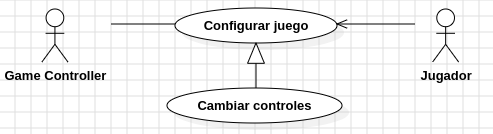
\includegraphics[width=.75\textwidth]{img/casos/cambiar_controles.png}}
		\caption{Caso de uso: Cambiar controles}
		\label{diagrama: caso: cambiar_controles}
	\end{figure}
	
	\begin{table}[H]
		\centering
		\begin{tabularx}{\textwidth}{|p{0.3\textwidth}|p{0.3\textwidth}|p{0.3\textwidth}|}
			\hline
			\textbf{CASO DE USO} & \multicolumn{2}{|l|}{Cambiar controles} \\ \hline
			
			\textbf{ACTOR} & \multicolumn{2}{|l|}{Jugador} \\ \hline
			
			\textbf{DESCRIPCIÓN} & \multicolumn{2}{|>{\raggedright\arraybackslash}X|}{El jugador configura los controles para las acciones del personaje.} \\ \hline
			
			\textbf{PRECONDICIÓN} & \multicolumn{2}{|l|}{Ninguna} \\ \hline
			
			\textbf{FLUJO BÁSICO} & \multicolumn{1}{|c|}{\textbf{ACTOR}} & \multicolumn{1}{|c|}{\textbf{SISTEMA} } \\ \hline
			& 
			1. Selecciona el menú de configuración. \newline
			3. Selecciona el sub menú de controles. \newline
			5. Selecciona una acción. \newline
			7. Presiona un botón en el tiempo dado. \
			&
			2. Muestra configuración de audio y de controles. \newline
			4. Muestra un listado de acciones y su botón/tecla asignada. \newline
			6. Inicia un contador esperando respuesta del jugador. \newline 
			8. Configura la acción al botón seleccionado. 
			 \\ \hline
			 
			 \textbf{FLUJO ALTERNO} & \multicolumn{1}{|c|}{\textbf{ACTOR}} & \multicolumn{1}{|c|}{\textbf{SISTEMA} } \\ \hline
			 1. Omisión.
			 & 
			 1. Selecciona el menú de configuración. \newline
			 3. Selecciona el sub menú de controles. \newline
			 5. Selecciona una acción. \newline
			 7. No presiona un botón en el tiempo dado. 
			 &
			 2. Muestra configuración de audio y de controles. \newline
			 4. Muestra un listado de acciones y su botón/tecla asignada. \newline
			 6. Inicia un contador esperando respuesta del jugador. \newline 
			 8. Mantiene la configuración actual de la acción. 
			 \\ \hline
			
			\textbf{POSTCONDICIÓN} & \multicolumn{2}{|l|}{Ninguna} \\ \hline
		\end{tabularx}
		\caption{Descripción del caso de uso: Cambiar controles}
		\label{table: caso: cambiar_controles}
	\end{table}
	
	%cambiar volumen
	\begin{figure}[H]
		\centering
		\fbox{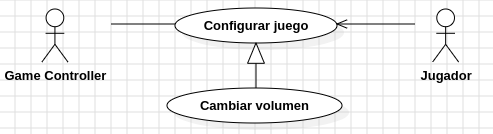
\includegraphics[width=.75\textwidth]{img/casos/cambiar_volumen.png}}
		\caption{Caso de uso: Cambiar volumen}
		\label{diagrama: caso: cambiar_volumen}
	\end{figure}
	
	\begin{table}[H]
		\centering
		\begin{tabularx}{\textwidth}{|p{0.3\textwidth}|p{0.3\textwidth}|p{0.3\textwidth}|}
			\hline
			\textbf{CASO DE USO} & \multicolumn{2}{|l|}{Cambiar volumen} \\ \hline
			
			\textbf{ACTOR} & \multicolumn{2}{|l|}{Jugador} \\ \hline
			
			\textbf{DESCRIPCIÓN} & \multicolumn{2}{|>{\raggedright\arraybackslash}X|}{Se configuran los volúmenes del juego} \\ \hline
			
			\textbf{PRECONDICIÓN} & \multicolumn{2}{|l|}{Ninguna} \\ \hline
			
			\textbf{FLUJO BÁSICO} & \multicolumn{1}{|c|}{\textbf{ACTOR}} & \multicolumn{1}{|c|}{\textbf{SISTEMA} } \\ \hline
			&
			1. Selecciona el menú de configuración. \newline
			3. Selecciona el sub menú de volumen. \newline
			5. Selecciona y desplaza la barra de volumen especifica. 
			& 
			2. Muestra configuración de audio y de controles. \newline
			4. Muestra barras deslizables de volumen. \newline
			6. Actualiza el volumen seleccionado. 
			\\ \hline
			
			\textbf{POSTCONDICIÓN} & \multicolumn{2}{|l|}{Ninguna} \\ \hline
		\end{tabularx}
		\caption{Descripción del caso de uso: Cambiar volumen}
		\label{table: caso: cambiar_volumen}
	\end{table}
	
	% Cambiar modo
	\begin{figure}[H]
		\centering
		\fbox{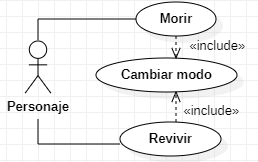
\includegraphics[width=.5\textwidth]{img/casos/cambiar_modo.png}}
		\caption{Caso de uso: Cambiar modo}
		\label{diagrama: caso: cambiar_modo}
	\end{figure}
	
	\begin{table}[H]
		\centering
		\begin{tabularx}{\textwidth}{|p{0.3\textwidth}|p{0.3\textwidth}|p{0.3\textwidth}|}
			\hline
			\textbf{CASO DE USO} & \multicolumn{2}{|l|}{Cambiar modo} \\ \hline
			
			\textbf{ACTOR} & \multicolumn{2}{|l|}{Personaje (Jugador)} \\ \hline
			
			\textbf{DESCRIPCIÓN} & \multicolumn{2}{|>{\raggedright\arraybackslash}X|}{El personaje tiene un segundo intento después de morir y lo recupera cuando revive} \\ \hline
			
			\textbf{PRECONDICIÓN} & \multicolumn{2}{|l|}{Morir o Revivir} \\ \hline
			
			\textbf{FLUJO BÁSICO} & \multicolumn{1}{|c|}{\textbf{ACTOR}} & \multicolumn{1}{|c|}{\textbf{SISTEMA} } \\ \hline
			&
			1. El personaje muere. \newline 
			2. El personaje encuentra el lugar donde falleció. 
			& 
			2. El personaje reaparece con el ultimo NPC con el que interactuó (Sus estadísticas están determinadas por el flujo conversacional del NPC) en modo `Afterlife'. \newline
			3. El personaje recupera sus estadísticas iniciales y continua el juego. 
			\\ \hline
			
			\textbf{FLUJO ALTERNO} & \multicolumn{1}{|c|}{\textbf{ACTOR}} & \multicolumn{1}{|c|}{\textbf{SISTEMA} } \\ \hline
			1. El jugador fallece en modo `Afterlife'.
			&
			1. El personaje muere. \newline 
			2. El personaje muere nuevamente. 
			& 
			2. El personaje reaparece con el ultimo NPC con el que interactuó en modo `Afterlife'. \newline
			3. El personaje reaparece en el `respawn'.
			\\ \hline
			
			\textbf{FLUJO ALTERNO} & \multicolumn{1}{|c|}{\textbf{ACTOR}} & \multicolumn{1}{|c|}{\textbf{SISTEMA} } \\ \hline
			1. El jugador no fallece en modo `Afterlife' y no encuentra donde falleció.
			&
			1. El personaje muere. \newline 
			2. El personaje sigue jugando en modo `Afterlife'.
			& 
			2. El personaje reaparece con el ultimo NPC con el que interactuó en modo `Afterlife'. \newline
			3. El personaje se mantiene en modo `Afterlife'.
			\\ \hline
			
			
			\textbf{POSTCONDICIÓN} & \multicolumn{2}{|l|}{Revivir o Morir} \\ \hline
		\end{tabularx}
		\caption{Descripción del caso de uso: Cambiar modo}
		\label{table: caso: cambiar_modo}
	\end{table}

	\clearpage
	\begin{figure}[H]
		\centering
		%	\fbox{\includegraphics[width=.75\textwidth]{img/casos/}}
		\caption{Caso de uso: }
		\label{diagrama: caso: }
	\end{figure}
	
	\begin{table}[H]
		\centering
		\begin{tabularx}{\textwidth}{|p{0.3\textwidth}|p{0.3\textwidth}|p{0.3\textwidth}|}
			\hline
			\textbf{CASO DE USO} & \multicolumn{2}{|l|}{} \\ \hline
			
			\textbf{ACTOR} & \multicolumn{2}{|l|}{} \\ \hline
			
			\textbf{DESCRIPCIÓN} & \multicolumn{2}{|>{\raggedright\arraybackslash}X|}{} \\ \hline
			
			\textbf{PRECONDICIÓN} & \multicolumn{2}{|l|}{} \\ \hline
			
			\textbf{FLUJO BÁSICO} & \multicolumn{1}{|c|}{\textbf{ACTOR}} & \multicolumn{1}{|c|}{\textbf{SISTEMA} } \\ \hline
			
			& & \\ \hline
			
			\textbf{POSTCONDICIÓN} & \multicolumn{2}{|l|}{} \\ \hline
		\end{tabularx}
		\caption{Descripción del caso de uso: }
		\label{table: caso: }
	\end{table}
	
	\subsection{Diagrama de clases}

	\subsection{Diagrama de secuencia}

	\subsection{Diagrama de estados}

	\subsection{Diagrama de actividades}

	\clearpage
	
	\section{Referencias Bibliográficas}
	
	\begin{thebibliography}{10}
	
	%Estado del arte
	\bibitem{game:hades}
	Supergiant Games, \textit{Hades}. Supergiant Games 2019.
	
	\bibitem{game:celeste}
	Maddy Makes Games , \textit{Celeste}. Maddy Makes Games, 2018.
	
	\bibitem{game:hollow}
	Team Cherry, \textit{Hollow Knight}, Team Cherry, 2017.
	
	\bibitem{game: coffee}
	Toge Productions, \textit{Coffee Talk}, Toge Productions, 2020.
	
	\bibitem{app: character}
	Character Technologies, Inc. ``character.ai'', 2022. [En línea]. Disponible: \url{https://character.ai}.  [Accedido: 11-Junio-2024].

	\bibitem{app: unity}
	Unity Technologies. ``Unity para principiantes | Unity''. Unity. 4. [En línea]. Disponible: \url{ttps://unity.com/es/learn/get-started} [Accedido el 13 de junio de 2024].

	\bibitem{lan: c_sharp}
	E. Canle Fernández. ``¿Qué lenguaje de programación usa Unity? – Tokio School”. Tokio School. [En línea]. Disponible: \url{https://www.tokioschool.com/noticias/lenguaje-unity/#:~:text=C#,%20que%20se%20pronuncia%20'C,sistema%20de%20programación%20por%20eventos}. [Accedido el 13 de junio de 2024].

	\bibitem{lan: prolog}
	UNAM. ``PROLOG `'. [En línea]. Disponible: \url{https://virtual.cuautitlan.unam.mx/intar/?page_id=212#:~:text=PROLOG%20utiliza%20un%20lenguaje%20basado,lógica%20partiendo%20de%20predicados%20determinados}. [Accedido el 13 de junio de 2024].

	\bibitem{lan: mongo}
	MongoDB. ``MongoDB: The Developer Data Platform''. MongoDB.  [En línea]. Disponible: \url{https://www.mongodb.com}. [Accedido el 13 de junio de 2024].

	\bibitem{app: star}
	MKLab.  ``StarUML''. StarUML. [En línea]. Disponible: \url{https://www.pixilart.com}. [Accedido el 13 de junio de 2024].
	
	\bibitem{app: pixilart}
	Pixilart.  ``Pixilart''. Pixilart LLC. [En línea]. Disponible: \url{https://staruml.io}. [Accedido el 13 de junio de 2024].

	\end{thebibliography}
	
\end{document}

